\chapter{Information System}
 
\section{Information System structure}
AllSpark is an enterprise which is involved deeply in the Information Technology and its Information System structure is articulated in order to efficiently face the works thanking the gathered in the job sector.

Since the digital technology reach each task of the Company, a lot of operations are thought to be performed through the automatic management except for the ones that need the human supervision due the critical objective such as business operations. 

The Information System structure base its functionality on six independent server that are charged to satisfy functions for a defined close context and several independent lightweight computers adopted by the personal that use the servers provide functionalities. This is a modularization of the working load to improve efficiency and reliability.

The six servers are represented in figure \ref{2img:NetMap} and follow described:
\begin{description}
\item[Administrative Server:] is the main server for the Company's lifecycle operations. This is the core of the aggregated functionalities such as the Business operations, the high level resource management and authority identification.
\item[Project Support Server:] aims to furnish the best services to developers regrouping data, resources and services used during the Project development. The unique scope of this machine is to supply each needing of Projects.
\item[Accounting Server:] tracks the users' public information such as their presence and their basic information unsed by the System to recognize them inside the Company and give the relative authorizations.
\item[File Server:] is the core of AllSpark's data storage which contains all kind of data used by the Company comprehensive the historical data and the supporting data for the Administrative Server. 
\item[Customer Accounting Server:] it stores a series of informations of customers in order to be reused by the business. In particular it store data about the customer identity, products bought and commercial relevance data about relation with AllSpark.
\item[Financial Server:] reserves all its work to the management of business activities that need to be separated from others system to avoid possible data corruption.
\end{description}

\begin{figure}
\begin{centering}
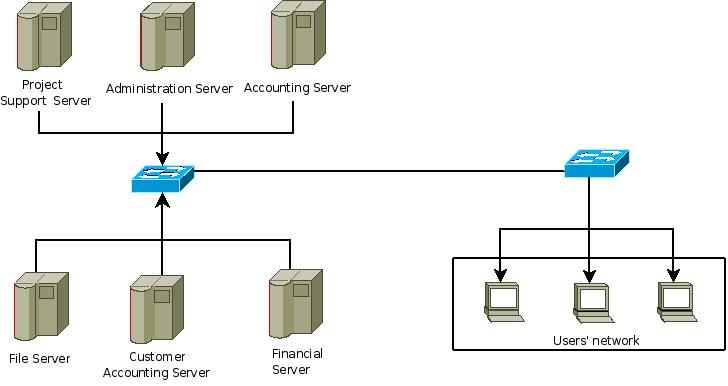
\includegraphics[scale=0.45]{assign3/dia/NetMap.jpeg}
\caption{AllSpark Network Map.}
\label{2img:NetMap}
\end{centering}
\end{figure}


\section{Use case diagrams}
The AllSpark Information System foresee several actors that are involved to and are represented in the following diagrams. Each actor represent a single entity or a general one such as the ``Secretary'' who describe several complementary people.

The functions are pretty isolated since the structure has been thought to be modular in the scope to be robust and in particular for each area described in \ref{2img:cmap} there is a use case; the Research and Development area does not have a different kind of informations with respect the Project and so is treated as it. In order to be clear each server functionality group together several use case that are ordered as independent functions for a single server.
 
 
\subsection{Administrative}
\begin{figure}
\begin{centering}
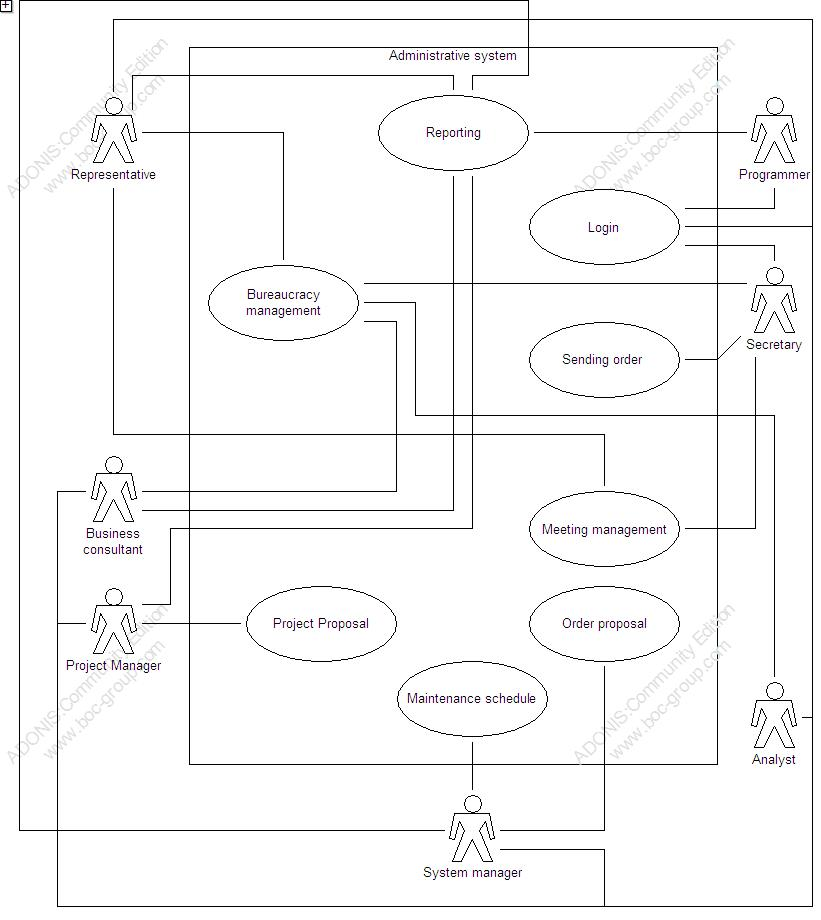
\includegraphics[scale=0.45]{assign3/adonis/imgs/administrative.jpg}
\caption{AllSpark Administrative use case.}
\label{2img:[use]administrative}
\end{centering}
\end{figure}

\subsection{Project}
\begin{figure}
\begin{centering}
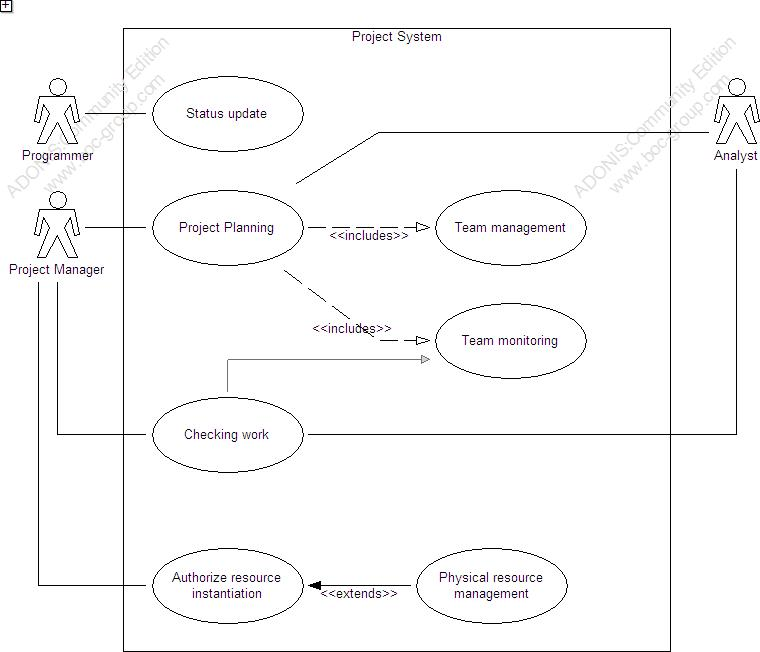
\includegraphics[scale=0.45]{assign3/adonis/imgs/project.jpg}
\caption{AllSpark Project use case.}
\label{2img:[use]project}
\end{centering}
\end{figure}

\subsection{Course}
\begin{figure}
\begin{centering}
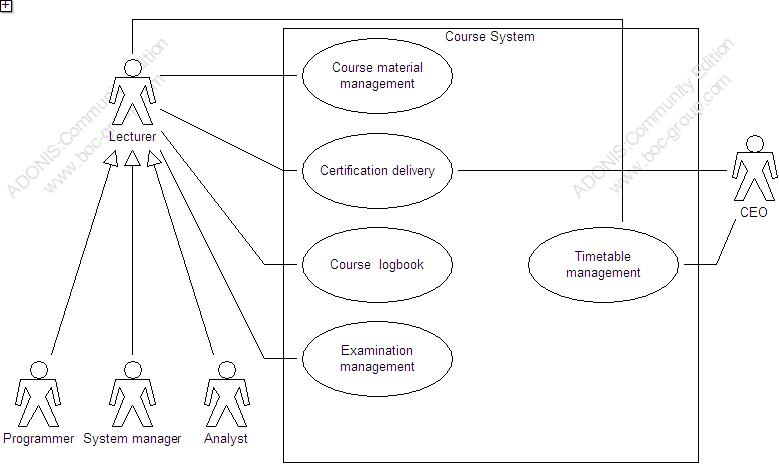
\includegraphics[scale=0.45]{assign3/adonis/imgs/course.jpg}
\caption{AllSpark Course use case.}
\label{2img:[use]Course}
\end{centering}
\end{figure}

\subsection{Commercial}
\begin{figure}
\begin{centering}
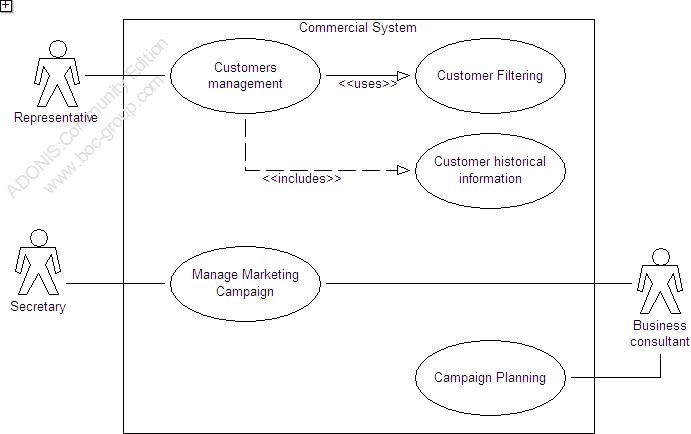
\includegraphics[scale=0.45]{assign3/adonis/imgs/commercial.jpg}
\caption{AllSpark Commercial use case.}
\label{2img:[use]commercial}
\end{centering}
\end{figure}

\subsection{Resource}
\begin{figure}
\begin{centering}
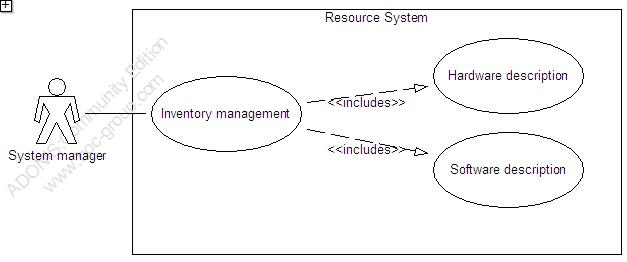
\includegraphics[scale=0.45]{assign3/adonis/imgs/resource.jpg}
\caption{AllSpark use case representing the Resource management.}
\label{2img:[use]resource}
\end{centering}
\end{figure}

\subsection{Documentation}
\begin{figure}
\begin{centering}
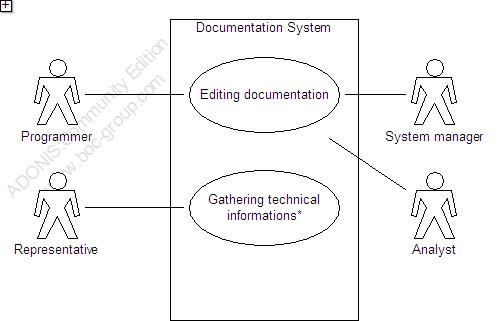
\includegraphics[scale=0.45]{assign3/adonis/imgs/documentation.jpg}
\caption{AllSpark Documentation management use case.}
\label{2img:[use]documentation}
\end{centering}
\end{figure}
\section{DataBase design}
In this section is presented the structure of the database which supports
the activities of the AllSpark organization.
In order to provide a more clear picture of the structure the database is
divided in different sections. 

Each one of this supports a different section of the organization, briefly
they are:
\begin{description}
\item[Administration: ] Provide support for the employees, projects and
customer organization.
\item[Project: ] Here are stored all the information of the projects on
which the organization is working.
\item[Resources: ] This part provides support for hosting the resources of
the enterprise, such as documentation, project details.
\end{description}

\subsection{Administrative section}
This section of the information system provides support for the
administrative part of AllSpark organization.
In particular it handles the employees administration, with their
specialization and roles. The activity classes permits to track a log of
each worker activity and to plan future event as meetings or deadlines.

Moreover it manages the inventory of the organization, which is mainly
composed by software and hardware (servers, network infrastructures). It
contains the references to the suppliers list, in order to retrieve
informations who supplied each item used in the organization.

In this part of the database is stored even the customer and their
relative contracts details. The image in \ref{3img:classadmin} shows the
details of this database in the form of a class diagram.

\begin{figure}[H]
\centering
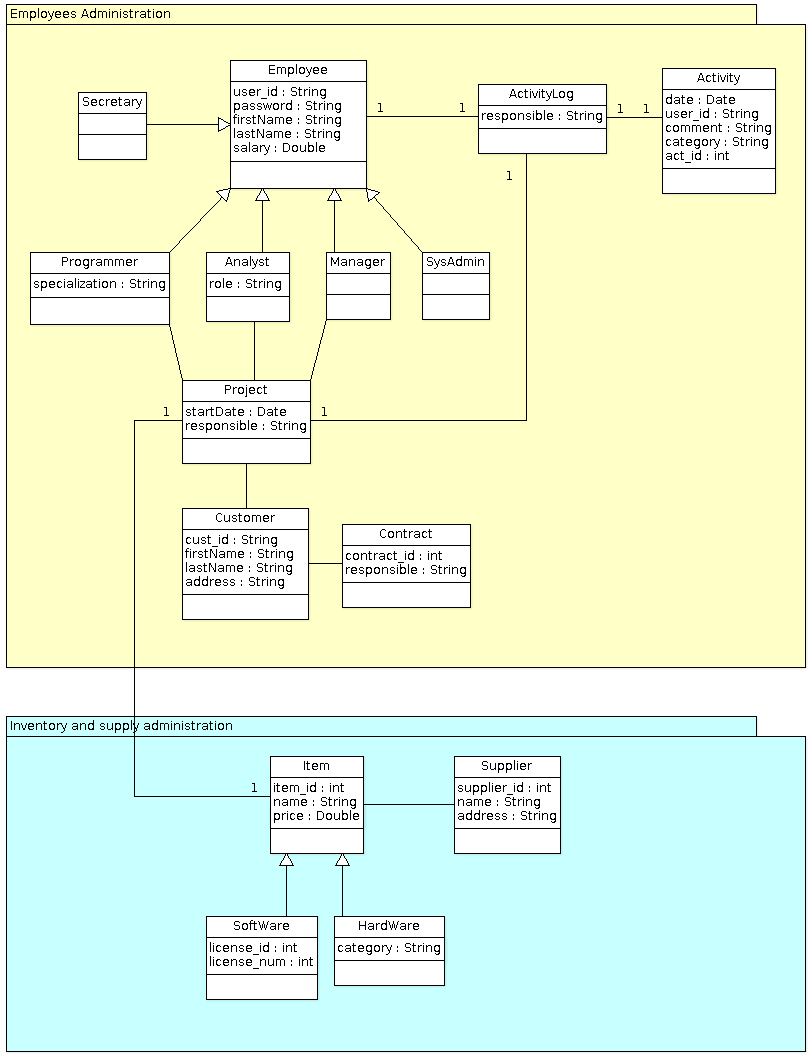
\includegraphics[scale=0.50]{assign3/argo/imgs/administrative.png}
\caption{Class diagram describing the administration database}
\label{3img:classadmin}
\end{figure}

\subsection{Project Section}
The branch of the database which manages the handling of the data related
to the projects is depicted in figure \ref{3img:classprj}.
One of the relevant thing is the managing of the budget specific for each
project, In fact every resource used for the project, which often is an
hardware resource or an intervention of technical assistance (internal or
external), is accounted on the project budget.

Other parts of the database maintain the informations about the various
teams which cooperates in the project, specifying their roles and members.
For a human resource point of view, the actors involved in a project
lifecycle are usually a manager and a variable number of developers and
analysts. 

The case of a research project falls into the general definition of a
common project, effectively, from a data point of view, there are no
relevant differences between the two kind of projects.

\begin{figure}[H]
\centering
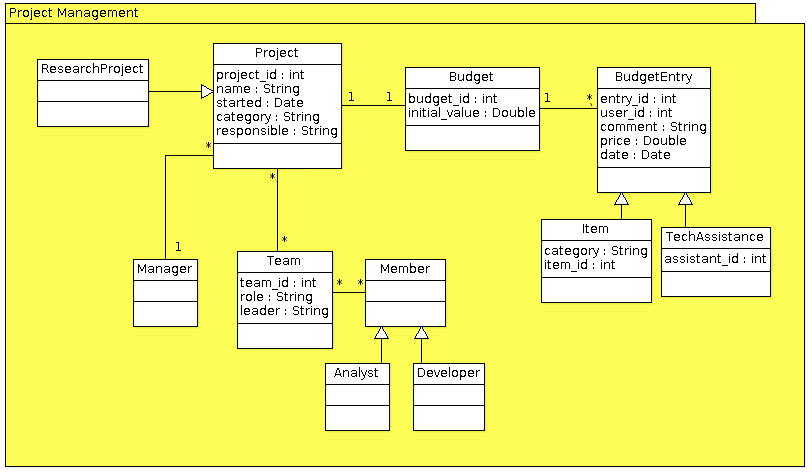
\includegraphics[scale=0.50]{assign3/argo/imgs/project.png}
\caption{Class diagram describing the project branch of the database}
\label{3img:classprj}
\end{figure}


